\documentclass[a4paper,11pt]{article}
\usepackage{CJKutf8}
\usepackage{listings}
\usepackage{graphics}
\title{苏州大学 《操作系统 》课程试卷}
\date{}

\begin{document}
\begin{CJK*}{UTF8}{gbsn}

%\maketitle
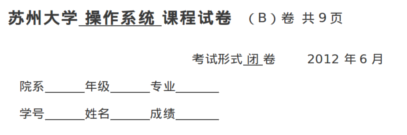
\includegraphics{headofpaperB.png}
\section{Linux命令及实际应用题}

\subsection{本题5分}
在线调查程序生成了文件\verb|fans.txt|, 其中记录的是每个球迷最喜欢的几位球星的名字, 格式为``球迷姓名\ \ 球星1\ \ 球星2 ...''.
其中每行所含的球星个数不固定. 现在需要用一条命令输出每个球星对应的球迷个数。例如若fans.txt内容为:
\begin{verbatim}
    chenjian 	戈麦斯 舍甫琴科
    chenbing 	托雷斯 法布雷加斯
    luchengtao  曼德祖基奇
    wangxin 	舍甫琴科 曼德祖基奇
    baicong	托雷斯
    liupeng	戈麦斯 德萨戈耶夫
\end{verbatim}
则输出结果为:
\begin{verbatim}
    戈麦斯: 2
    舍甫琴科: 2
    托雷斯: 2
    法布雷加斯: 1
    曼德祖基奇: 2
    德萨戈耶夫: 1
\end{verbatim}
请写出实现该功能的命令。
\\[1.5in]

\subsection{本题共10分}
文件\verb|scores.txt|记录了某课程学生的平时成绩, 格式为: 

学生姓名\ \ 第1次成绩\ \  第2次成绩\ \ 第3次成绩

\noindent 要实现以下功能:
\begin{enumerate}
\item (2分) 打印出第3次平时成绩不及格(低于60分)的所有同学的姓名.
\item (4分) 打印出第1次平时成绩最高分的同学姓名及成绩(仅打印一位同学即可, 不需考虑并列成绩).
\item (4分) 如果3次平时成绩的权重分别为0.2, 0.3, 0.5. 请用一条命令输出每位同学的加权平时成绩,格式为`姓名\ \ 加权成绩'.
\end{enumerate}
请分别写出相应命令.
\\[1.5in]

\subsection{本题5分}
已知当前目录下有7个子目录, 名称分别为lecture1 ... lecture7. 每个目录下均有若干类型的文件(例如PDF, TXT, DOC).
要实现下述效果:
\begin{enumerate}
\item 创建名为\verb|all_PDFs|的目录.
\item 将\verb|lecture1| ... \verb|lecture7|目录中所有PDF文件拷贝到目录\verb|all_PDFs|中.
\item 把目录\verb|all_PDFs|打包成名为\verb|all_PDFs.tar|的文件.
\item 把文件\verb|all_PDFs.tar|压缩成文件\verb|all_PDFs.tar.bz2|
\item 把\verb|all_PDFs.tar.bz2|解压 
\end{enumerate}
分别写出相应命令.
\\[1.5in]

\section{计算题}
\subsection{本题共10分}
在32位机器上, 假设页面大小为4096字节, 采用两级分页技术, 其中32位二进制地址中最高10位用于索引第一级页表,
中间10位用于索引第二级页表. 某进程被分配到的虚拟地址空间为第\verb|0x20000000|字节到\verb|0x2007ffff|字节(包括两端点), 
请回答:
\begin{enumerate}
\item 该进程分配到的虚拟地址空间一共是多少字节? 
\item 这些空间需要多少页面存放? 
\item 如果每个页表项占4字节, 该进程的页表共占多少字节? (一级页表和二级页表都考虑在内)
\item 如果采用一级分页技术, 最高20位用于索引页表, 最低12位用于表示页内偏移, 则该进程的页表共占多少字节?
\item 给定地址\verb|0x20012001|, 该地址对应一级页表中的第几个页表项? 二级页表中第几个页表项?
\end{enumerate}
注意: 你的答案均需用十进制表示.
\\[2in]


\subsection{本题15分}
某UNIX操作系统采用i-node节点记录文件在存储介质上的存放位置. 其中, 存储介质每数据块大小为4K, 又假设所有的指针均占用4个字节.
请结合下图回答以下问题:
\begin{enumerate}
\item `direct blocks'共容纳12个指针, 这些指针对应的存储区域一共是多少字节?
\item `single direct'指针对应的存储区域是多少个字节?
\item `double direct'指针对应的存储区域是多少字节?
\item `triple direct'指针对应的存储区域是多少字节?
\item 就该图所示的i-node节点而言, 存放文件属性的区域一共占据多少字节?
\end{enumerate}
 
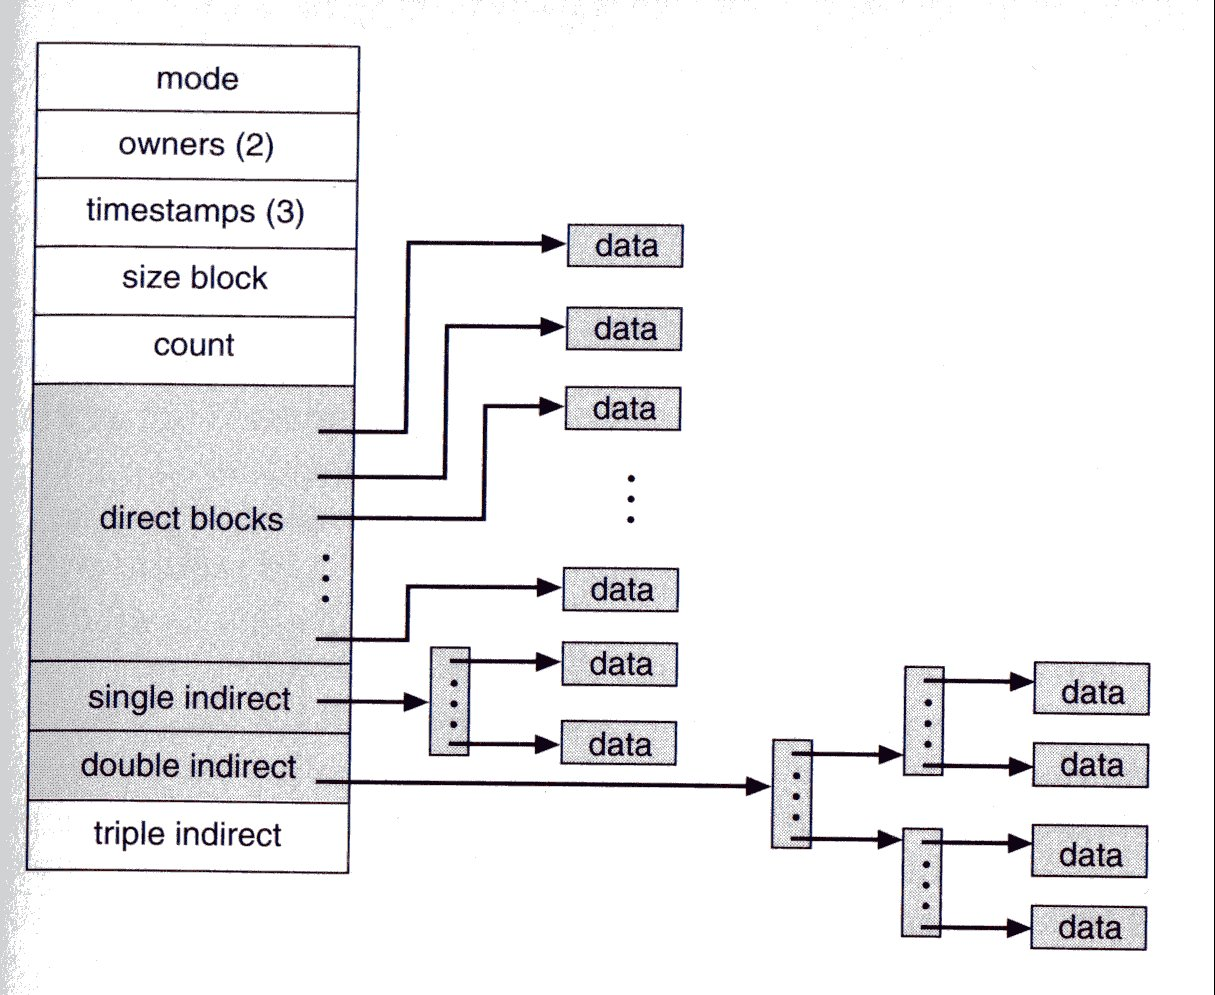
\includegraphics{inode-detail.jpg}
\\[2in]

\newpage
\section{Linux内核源代码题}
\subsection{本题8分}
请在标注``填空''的地方填写正确的函数调用参数. 注意阅读代码注释.

\begin{verbatim}
struct list_head {
    struct list_head *next, *prev;
};

static inline void __list_add(struct list_head *new,
                  struct list_head *prev,
                  struct list_head *next)
{
    next->prev = new;
    new->next = next;
    new->prev = prev;
    prev->next = new;
}

/**
 * list_add - add a new entry
 * @new: new entry to be added
 * @head: list head to add it after
 *
 * Insert a new entry after the specified head.
 * This is good for implementing stacks.
 */
static inline void list_add(struct list_head *new, struct list_head *head)
{
    __list_add(new, __________, __________);    /* 填空 */
}

/**
 * list_add_tail - add a new entry
 * @new: new entry to be added
 * @head: list head to add it before
 *
 * Insert a new entry before the specified head.
 * This is useful for implementing queues.
 */
static inline void list_add_tail(struct list_head *new, struct list_head *head)
{
    __list_add(new, __________, __________);   /* 填空 */
}

\end{verbatim}

%\newpage
\subsection{本题12分}
请在标注``填空''的地方填写正确的语句, 并画出\verb|__list_splice|操作的示意图.
注意阅读代码注释.
\begin{verbatim}
static inline void __list_splice(struct list_head *list,
                 struct list_head *head)
{
    struct list_head *first = list->next;
    struct list_head *last = list->prev;
    struct list_head *at = head->next;

    first->prev = head;

    _______________________;   /* 填空 */

    last->next = at;

    _______________________;   /* 填空 */
}

/**
 * list_splice - join two lists
 * @list: the new list to add.
 * @head: the place to add it in the first list.
 */
static inline void list_splice(struct list_head *list, struct list_head *head)
{
    if (!list_empty(list))
        __list_splice(list, head);
}

\end{verbatim}


\newpage
\subsection{本题10分}
Linux内核中的宏\verb|list_for_each|用于遍历双向循环链表. 以下代码段(功能是找出表\verb|list|中满足某条件的进程)演示了其具体用法:
\begin{verbatim}
struct list_head *p;

list_for_each(p, &list) {
    if (condition(p))  
        return list_entry(p, struct task_struct, run_list);
}

return NULL;
\end{verbatim}
又已知在Linux进程描述符结构中定义了以下字段用于构建进程间父子及兄弟关系:
\begin{verbatim}
struct task_struct {
    ...
    struct task_struct *parent; 
    struct list_head children; 
    struct list_head sibling; 
    ...
};
\end{verbatim}

这些关系可用下图表示:

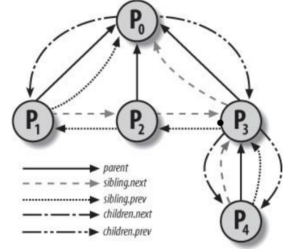
\includegraphics{parent4.png}

请综合上述给定信息, 写一个函数\verb|print_IDs_of_all_children(struct task_struct *p)|,
其功能是打印进程\verb|p|的所有子进程的ID. 要求写出包括函数返回类型在内的完整函数定义.
\\[3in]
%\newpage
\subsection{本题10分}
Linux内核中大量使用了散列表(哈希表)这种数据结构. 其中哈希函数的设计等价于以下代码:
\begin{verbatim}
unsigned long hash_long(unsigned long val, unsigned int bits)
{
    unsigned long hash = val * 0x9e370001UL;
    return hash >> (32 - bits);
}
\end{verbatim}
请回答: 上述函数中的参数\verb|bits|起什么作用? 如果某哈希表长度为1024个元素, 则调用函数\verb|hash_long|时,
参数\verb|bits|应该是多少?
\\[1.5in]

\section{简答题}
\subsection{本题5分}
采用连续存储方式记录文件在存储介质上的存放位置有什么优缺点?
在什么情况下连续存储方式是最理想的解决方案?
\\[1in]


\subsection{本题5分}
请说明磁盘的第0扇区内存放的两类重要内容及每类内容的作用.
\\[1in]

\subsection{本题5分}
请从至少两个角度说明为什么Linux内核源代码不能使用C标准库函数和头文件提供的功能.
\\[1.5in]

\end{CJK*}
\end{document}

